\begin{figure}
    \centering
    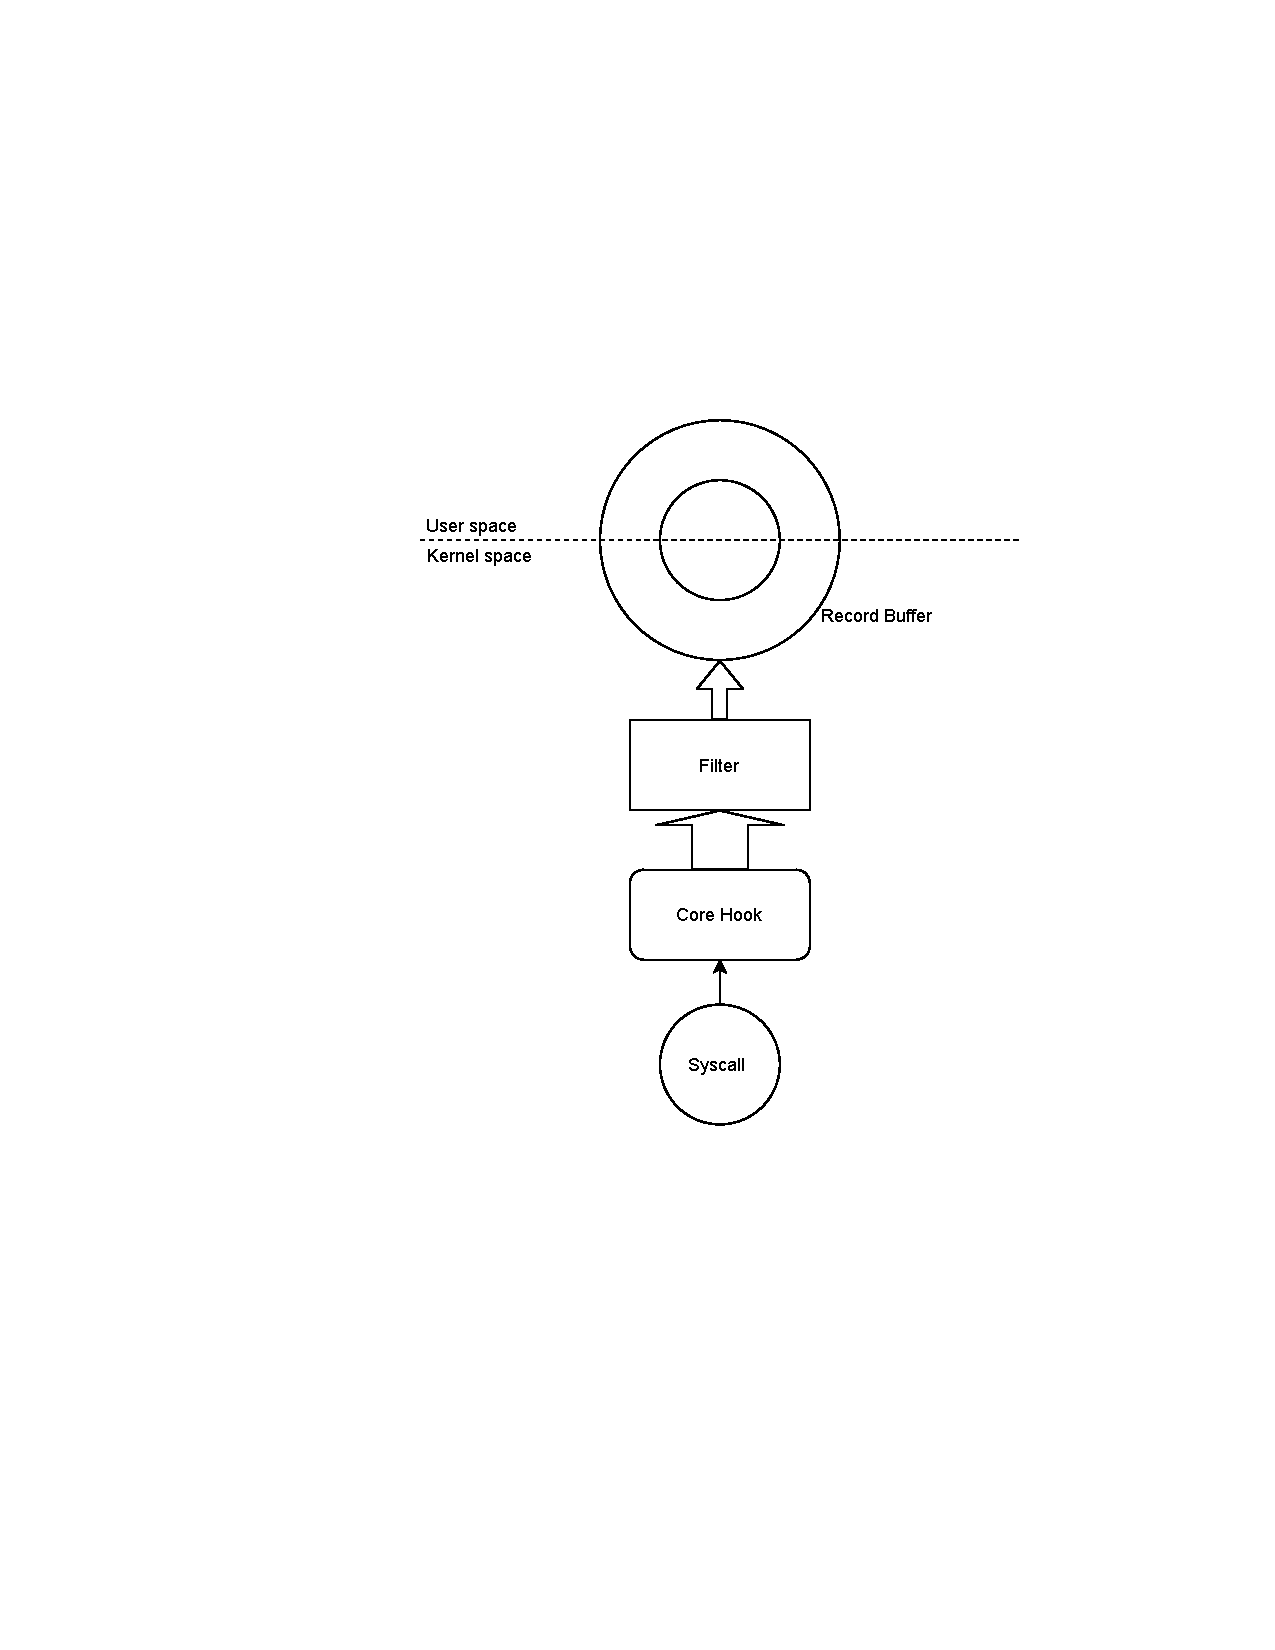
\includegraphics[width=0.5\textwidth]{figures/arch.pdf}
    \caption{The three parts of \$\{PROJECT\_NAME\}}
    \label{fig:arch}
\end{figure}


\section{Design}

% In this section, I describe the desgin of \$\{PROJECT\_NAME\} by focusing on how it solves the above challenges

In this section, I present the desgin of \$\{PROJECT\_NAME\} by focusing on how it addresses the above three key challenges. \$\{PROJECT\_NAME\} contians three parts: \textit{core hook}, \textit{filter}, and \textit{record transfer}. 

As Figure \ref{fig:arch} shows, in the kernel space, \textit{core hook} will firslty inspect each syscall and then transfer relevant information to \textit{filter} part. Subsequently, at the \textit{filter} part, syscall records with specific features (e.g., process id or name) will be selected and finally pass to \textit{record transfer}. Meanwhile, a daemon will check the buffer periodically and dump these data form buffer to file.

\begin{figure}
    \centering
    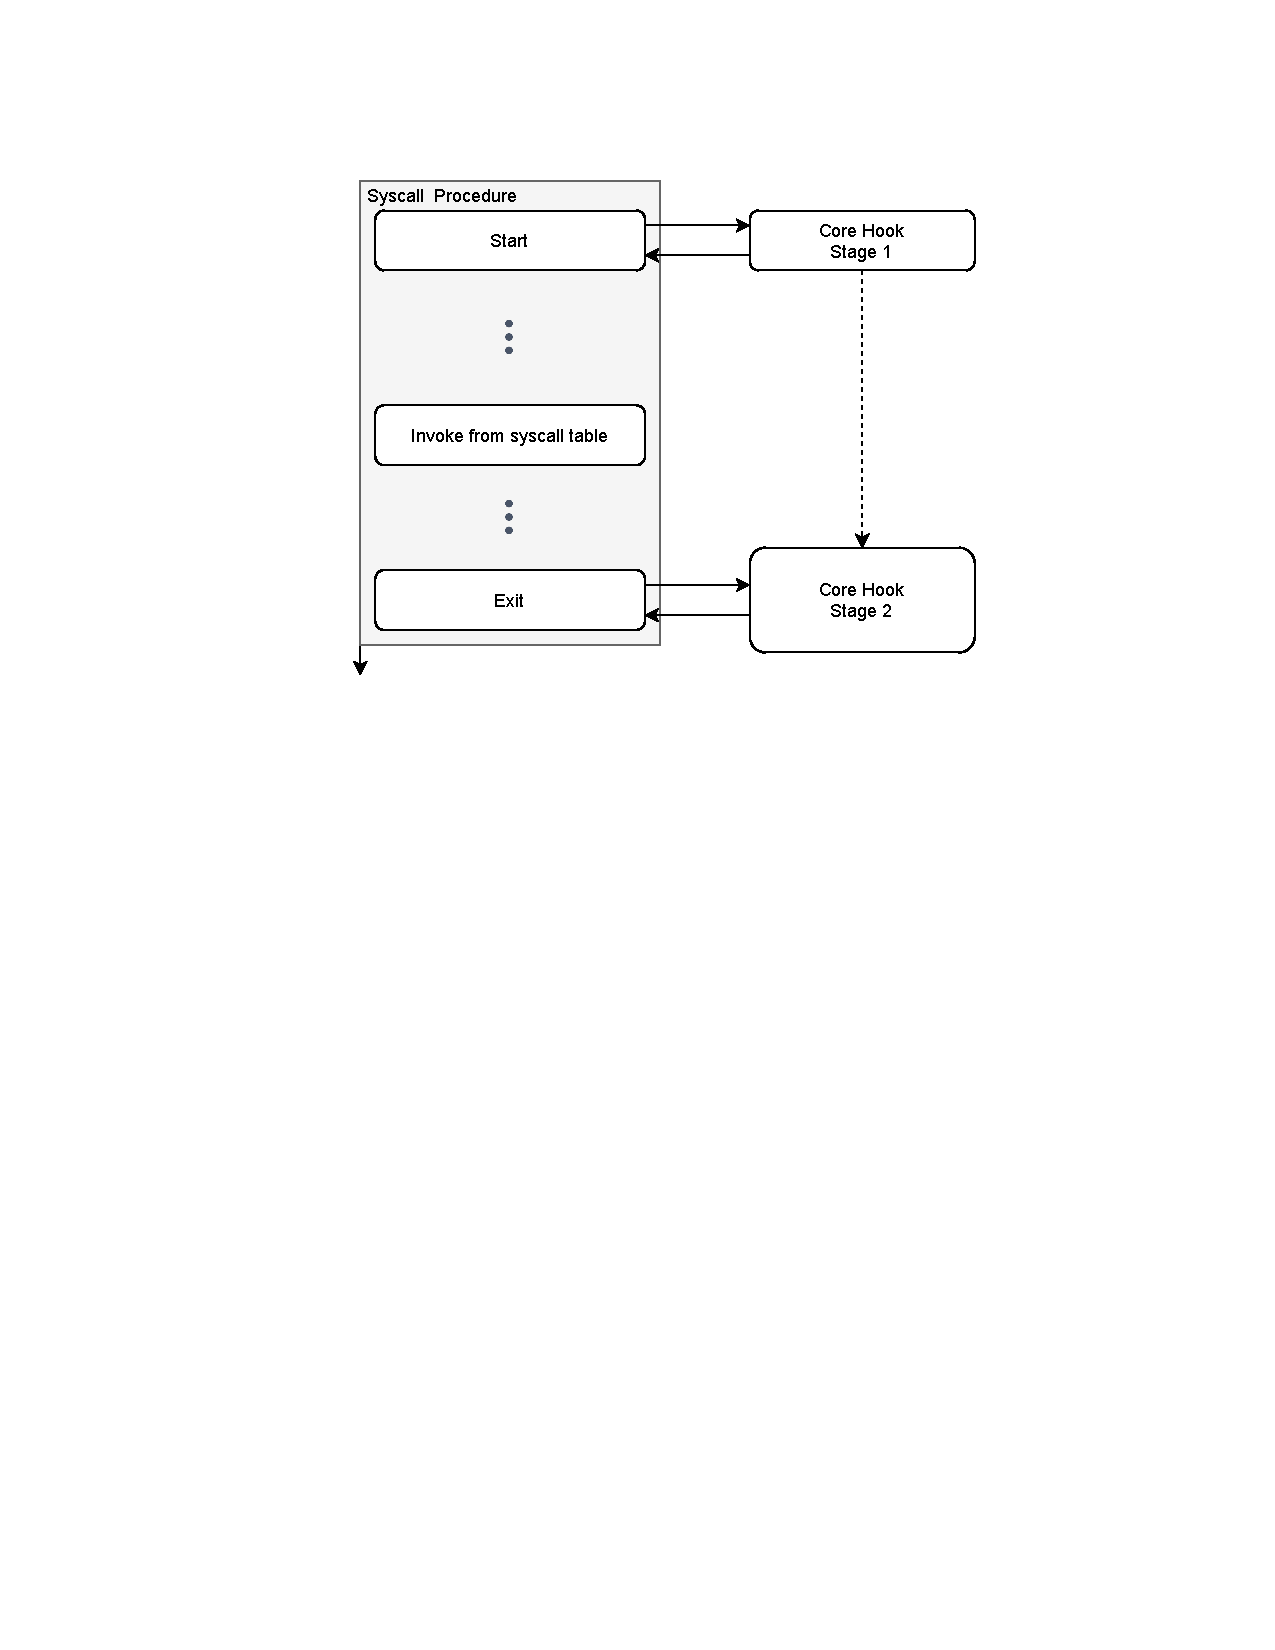
\includegraphics[width=0.5\textwidth]{figures/core-hook-desgin.pdf}
    \caption{The two tages of \textit{core hook}}
    \label{fig:core-hook-desgin}
\end{figure}


\subsection{Core Hook}

Figure \ref{fig:core-hook-desgin} shows the general workflow of \textit{core hook}. It consists of two stages of hooks, at the beginning and end of kernel handling of syscall. For the stage 1, \$\{PROJECT\_NAME\} will follow the start of syscall handlers and save the value of first parameter, if this syscall may change the memory addressed by first argument.


The second stage takes on more responsibility, including the recording of other pointer type parameters (except for the first one), and return values. Besides, this stage should also get the relevant information collected by stage 1.

There is still a problem that, due to the concurrency of the system, there may be multiple system calls being processed at the same time. Especially considering that the system calls processed in a relatively long period. So, there will be multiple system calls going to different stages of  \textit{core hook}.

This problem is solved by the observation that syscall will block the thread in user space. Therefore, we can find a one-to-one mapping from thread number to a system call event at any moment. I maintain a table to save these correspondences in second stage, and also get its first parameters from stage 1.

\subsection{Filter}

The \texttt{filter} part is a relatively simple component that requires information about the caller of the syscall from the Linux kernel. Then it will perform filter by pre-passed conditions. Last, it passes this filtered information on to the next part.

\subsection{Record Buffer}

The \textit{record buffer} is intended to act as a transit between kernel space and user space. Therefore it has two parts located in kernel space and user space respectively. One of the simplest designs is to maintain a daemon in user space constantly querying and retrieving the data stored in the buffer, and then dumping the data to a file. However, we note that this introduces a huge amount of overhead, mainly due to frequent file io. Placing a larger buffer in user space would also solve this problem, but \$\{PROJECT\_NAME\} do not want to introduce a large impact on the entire system.

Therefore, \textit{record buffer} is designed to keep fetching the buffer occupancy, and then dumps the whole buffer only after finding that the buffer occupancy has reached a threshold.